% =====================================================================
% Predictive Weight Optimization: A Machine Learning Approach to
% Maximizing Expected Value in Men's March Madness Brackets
% MAT-210 Mathematical Modeling, Davidson College, Spring 2026
%
% NOTE: This document references five figure files in a `figures/`
% subdirectory:
%   figures/reliability.png
%   figures/round_importance.png
%   figures/backtest.png
%   figures/reach_2026.png
%   figures/strategy_2026.png
% Upload these to your Overleaf project, or comment out the
% \includegraphics lines if you don't want to embed them yet.
% =====================================================================

\documentclass[12pt]{article}

\usepackage[utf8]{inputenc}
\usepackage[T1]{fontenc}
\usepackage[margin=1in]{geometry}
\usepackage{amsmath,amssymb,amsfonts}
\usepackage{bm}
\usepackage{booktabs}
\usepackage{graphicx}
\usepackage{float}
\usepackage{caption}
\usepackage{enumitem}
\usepackage{microtype}
\usepackage{hyperref}
\usepackage{xurl}

\hypersetup{
    colorlinks=true,
    linkcolor=black,
    citecolor=black,
    urlcolor=blue,
}

\title{Predictive Weight Optimization: A Machine Learning Approach to Maximizing Expected Value in Men's March Madness Brackets}
\author{Bryce Clement \and Christian Rutherford \and Devon Diaco}
\date{MAT-210 Mathematical Modeling, Davidson College, Spring 2026 \\ Prof.\ Tim Chartier}

\begin{document}

\maketitle

\begin{abstract}
We model the NCAA Division I Men's Basketball Tournament as a 63-game probability tree, and formulate the problem of choosing a 64-team bracket which maximizes expected ESPN Tournament Challenge points. To do so, we (i) fit a logistic-regression win-probability model to fifteen seasons (2010-2026) of KenPom efficiency data and tournament results (excluding 2020) and (ii) vectorize a Monte Carlo bracket simulator. We compare 3 deterministic strategies: chalk-by-seed, chalk-by-model and EV-max. The full model achieves an $83.0\%$ accuracy and $0.410$ log-loss on leave-one-season-out cross-validation. Backtesting 15 seasons shows that the model bracket wins 13/15 matchups over the seed-chalk; its realized score has 428 more points (52\% relative improvement). In 2026, the model bracket scores 1{,}570 points to the seed-chalk's 1{,}000 points, and selects Michigan as champion with a 67.2\% probability.
\end{abstract}

\section{Problem Description}

In March, sixty-eight Division I men's basketball teams participate in a single-elimination tournament (sixty-four teams after the play-in ``First Four'') to determine the national champion. Tens of millions of fans complete a \emph{bracket}, their predictions of the winners of all sixty-three games before the tournament even starts. ESPN's Tournament Challenge alone collected over 26.6 million brackets in 2026~\cite{espn}, a record for the fourth consecutive year.

Picking a good bracket is difficult. In a single-elimination tournament, even the pre-tournament favorite has probability less than $25\%$~\cite{kenpom} of winning all six games. The scoring is also non-linear: ESPN assigns 10, 20, 40, 80, 160, and 320 points, respectively, to the R64, R32, S16, E8, F4, and championship round games, so picking the champion is estimated to be worth 32 first round wins. Finally, the decision space is also very large: there are some $2^{63} \approx 9.2 \times 10^{18}$ possible brackets.

Note that per-game accuracy never maximizes expected total score since later rounds are worth far more points. This is a game where one does not maximize per-game accuracy, but rather expected total score.

\begin{quote}
\textbf{Goal.} We first build a calibrated win-probability model based on previous performance metrics, and then derive a rule for filling in the bracket that maximizes expected ESPN score under that model. We validate this model using all available NCAA tournaments from 2010 to 2026 with complete data.
\end{quote}

\section{Simplifications}

An entire model would include injuries, travel, officiating, the joint distribution of pool-entrant strategies, and prize structure. We make typical simplifications~\cite{lightgbm,lopezmatthews}.

\begin{itemize}[leftmargin=*]
\item \textbf{First Four excluded.} In modeling the 64-team bracket beginning with R64, we treat each First Four winner as their corresponding seed.
\item \textbf{Static, season-end features.} All KenPom features are static end-of-regular-season values; brackets are entered before any tournament games are played.
\item \textbf{Independent games.} Game results are conditionally independent given team attributes.
\item \textbf{Symmetric matchup framing.} Since each matchup is the signed difference of Team A's features from Team B's, $P(A\text{ beats }B) = 1 - P(B\text{ beats }A)$ by construction.
\item \textbf{Momentum from game logs, with a fallback proxy.} Late-season momentum is a decay-weighted win rate over a team's last 10 pre-tournament games (decay $0.85$); calculated from per-game schedule data scraped from Sports-Reference~\cite{sportsref}. For team-seasons without game-log coverage we fall back to an $\text{AdjEM} \times \text{Luck}$ proxy.
\item \textbf{Public-pick data is single-year.} ESPN's ``Who Picked Whom'' data was only available for 2019, meaning pool-relative analysis is theoretical (\S3.5) rather than backtested.
\item \textbf{2020 dropped from the backtest} (no tournament due to COVID).
\end{itemize}

\section{Mathematical Model}

\subsection{Win-probability oracle}

Let $\mathcal{T}_y$ denote the 64 tournament teams in year $y$. For each team $t\in\mathcal{T}_y$, we create 11 features by calculating 10 KenPom statistics: Adjusted Efficiency Margin (AdjEM), Adjusted Offensive Efficiency (AdjO), Adjusted Defensive Efficiency (AdjD), Adjusted Tempo (AdjT), Luck, two strength-of-schedule statistics (SOS-AdjEM and NCSOS-AdjEM), the decay-weighted Momentum signal of \S2, the Four Factors statistics offensive eFG\% (Off-eFG\%) and defensive eFG\% (Def-eFG\%), and a seed. For each ordered pair $(a, b)$ of teams, we define the signed feature difference
\begin{equation}
\Delta_{ab} = \mathbf{x}_y(a) - \mathbf{x}_y(b) \in \mathbb{R}^{11}, \qquad \Delta_{ab} = -\Delta_{ba}.
\end{equation}
We model the winning probability as
\begin{equation}
P_\theta(a\text{ beats }b) = \sigma\!\left(\theta_0 + \boldsymbol{\theta}^{\!\top} \Delta_{ab}\right) = \frac{1}{1 + \exp\!\big(-(\theta_0 + \boldsymbol{\theta}^{\!\top} \Delta_{ab})\big)},
\end{equation}
where $\sigma$ is the logistic function. It has the property that reversing the pair reverses $\Delta$, so $P_\theta(a, b) + P_\theta(b, a) = 1$. Following Lopez and Matthews~\cite{lopezmatthews} in this domain, we treat each game as a binary classification problem minimizing the log-loss.
\begin{equation}
\mathcal{L}(\boldsymbol{\theta}) = -\frac{1}{N}\sum_{i=1}^N \big[y_i \log \hat{p}_i + (1-y_i)\log(1-\hat{p}_i)\big],
\end{equation}
where $\hat p_i$ is the model's predicted probability of winning matchup $i$. Log-loss is the scoring rule of choice when the downstream task depends on calibrated probabilities.

\subsection{The bracket as a probability tree}

The bracket is a balanced binary tree of depth six, with 63 internal nodes (games) and 64 leaves (teams), four regions of 16 teams each, and a Final Four. Given $P_\theta$ it induces a joint distribution on the random vector $(R_t)_{t \in \mathcal{T}_y}$ where $R_t \in \{0,\dots,6\}$ is the maximum round reached by team $t$. This distribution is not factored because each team's path depends on the opponents it matches up against, so we estimate it by Monte Carlo (\S4.3).

\subsection{ESPN scoring and the EV objective}

A bracket entry $\pi = (\pi_R)_R$ indicates for each round $R$ which teams are picked to advance. The ESPN scoring rule is
\begin{equation}
S(\pi, R) = \sum_R w_R \cdot \#\{t \in \pi_R : R_t \ge \mathrm{idx}(R)\},\qquad w = (10, 20, 40, 80, 160, 320),
\end{equation}
with a maximum score of 1{,}920. Define the marginal reach probability $\rho_R(t) := \Pr[R_t \ge \mathrm{idx}(R)]$. The expected score is
\begin{equation}
\mathrm{EV}(\pi) = \sum_R w_R \sum_{t \in \pi_R} \rho_R(t).
\end{equation}
By the linearity of expectation, the EV-maximizing entry under a fixed model is the closed-form greedy rule: at every game, pick whichever reachable team has the higher $\rho_R$. In particular, there is no need to search over the $2^{63}$ bracket space. This is a key methodological observation of the project.

\subsection{Bracket strategies}

We enumerate three deterministic pick strategies:

\begin{enumerate}[leftmargin=*]
\item \textbf{chalk\_seed.} Pick the lower-seeded team in every game. Baseline.
\item \textbf{chalk\_model.} At every game, choose the action $\arg\max_c P_\theta(c\text{ wins})$.
\item \textbf{ev\_max.} For each game in round R compute $\arg\max_c \rho_R(c)$.
\end{enumerate}

For a calibrated symmetric model, chalk\_model and ev\_max coincide because respective per-game $\arg\max$s / reach-probability $\arg\max$s agree about which team to bet on. We confirm this empirically in \S5.4.

\subsection{The pool-percentile objective (theoretical extension)}

EV is not the right target; after Metrick~\cite{metrick}, we define a field of $M$ competitor brackets sampled from the public-pick distribution and a target percentile $\alpha$. The pool-finish probability is
\begin{equation}
\mathrm{PFP}_\alpha(\pi) = \Pr\!\left[\frac{1}{M}\sum_{i=1}^M \mathbf{1}\!\big[S(\pi, R) > S(\pi^{(i)}, R)\big] \ge \alpha\right].
\end{equation}
A natural heuristic is, for every game in $R \ge \mathrm{S16}$, choose the team $c$ maximizing $\rho_R(c)[1-q_R(c)]$, where $q_R(c)$ is the public pick rate. This leverages the model where it disagrees with the crowd. Since we only have one year of public-pick data, we do not include this approach in the backtest below.

\section{Solution}

\subsection{Training the win-probability model}

The matchup dataset has \textbf{2{,}014 rows} covering every actual tournament game played between 2010--2026~\cite{sportsref} (excluding 2020), with mirrored orderings yielding exact 50/50 class balance across the 1{,}007 games. In each LOSO training fold, we standardized the features. We validated models by leave-one-season-out cross-validation, as it better resembles the forecasting problem of training on past seasons to predict a future tournament.

\begin{table}[H]
\centering
\begin{tabular}{lrrrr}
\toprule
Model & Log-loss & Std & Accuracy & Brier \\
\midrule
Logistic, seed only & 0.572 & 0.046 & 70.5\% & 0.195 \\
\textbf{Logistic, full features} & \textbf{0.410} & \textbf{0.090} & \textbf{83.0\%} & \textbf{0.129} \\
XGBoost~\cite{xgboost} & 0.434 & 0.094 & 81.6\% & 0.135 \\
CatBoost~\cite{catboost} & 0.442 & 0.092 & 80.8\% & 0.137 \\
Random Forest~\cite{sklearn} & 0.471 & 0.060 & 78.3\% & 0.153 \\
LightGBM~\cite{lightgbm} & 0.518 & 0.140 & 81.2\% & 0.145 \\
\bottomrule
\end{tabular}
\caption{Model comparison under leave-one-season-out cross-validation.}
\end{table}

Full logistic regression achieves the best log-loss and Brier score, and so is used for downstream tasks. While tree ensembles achieve similar accuracy, they are worse at probability calibration, exactly the property we need to compute EV. Adding the ten KenPom features to the seed-only baseline reduces log-loss by $28\%$. Given the small number of ${\sim}2{,}000$ training rows, tree ensembles may not be able to capture the non-linearities successfully. The LightGBM high variance across folds also suggests the model is overfitting on the small per-season slices. In the reliability diagram in Figure~\ref{fig:reliability}, the predicted probabilities are well-calibrated, meaning that predictions closely track observed frequencies across the probability range.

\begin{figure}[H]
\centering
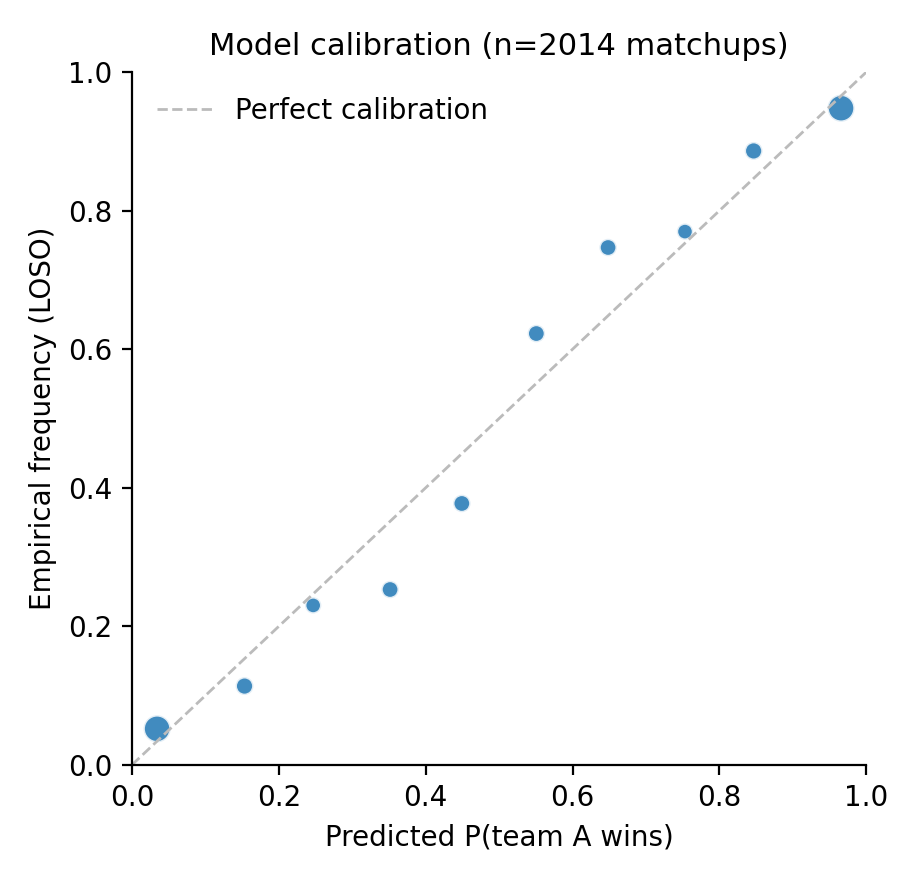
\includegraphics[width=0.7\textwidth]{figures/reliability.png}
\caption{Reliability (calibration) diagram for the full logistic model on 2{,}014 LOSO predictions across 2010--2026.}
\label{fig:reliability}
\end{figure}

\subsection{Fitted coefficients}

The features are standardized, making coefficients interpretable as effect sizes on the response.

\begin{table}[H]
\centering
\begin{tabular}{lr@{\hskip 1cm}lr}
\toprule
Feature & $\hat\theta$ & Feature & $\hat\theta$ \\
\midrule
d\_Seed & \textbf{+2.60} & d\_Momentum & $-0.65$ \\
d\_AdjEM & \textbf{+1.83} & d\_OffEFG & $-0.11$ \\
d\_AdjO & $+1.62$ & d\_NCSOS-AdjEM & $-0.06$ \\
d\_AdjD & $-1.42$ & d\_DefEFG & $+0.02$ \\
d\_SOS-AdjEM & $+1.36$ & d\_AdjT & $+0.02$ \\
d\_Luck & $+1.10$ & & \\
\bottomrule
\end{tabular}
\caption{Standardized logistic regression coefficients.}
\end{table}

These are sensible. Better teams (lower seeds) are more efficient (higher offensive rating, lower defensive rating), and play harder schedules, but tempo makes no difference. The Four Factors coefficients are all near zero due to multicollinearity with the adjusted efficiencies they are used to form. The Momentum coefficient is slightly negative because the decay-weighted winning percentage is correlated with efficiencies already in the model, and teams that get hot late in the year tend to regress during the tournament. Round-by-round fits (Figure~\ref{fig:rounds}) show the Momentum coefficient becoming increasingly negative through S16 and attenuating thereafter, with Seed and AdjEM as the primary contributors.

\begin{figure}[H]
\centering
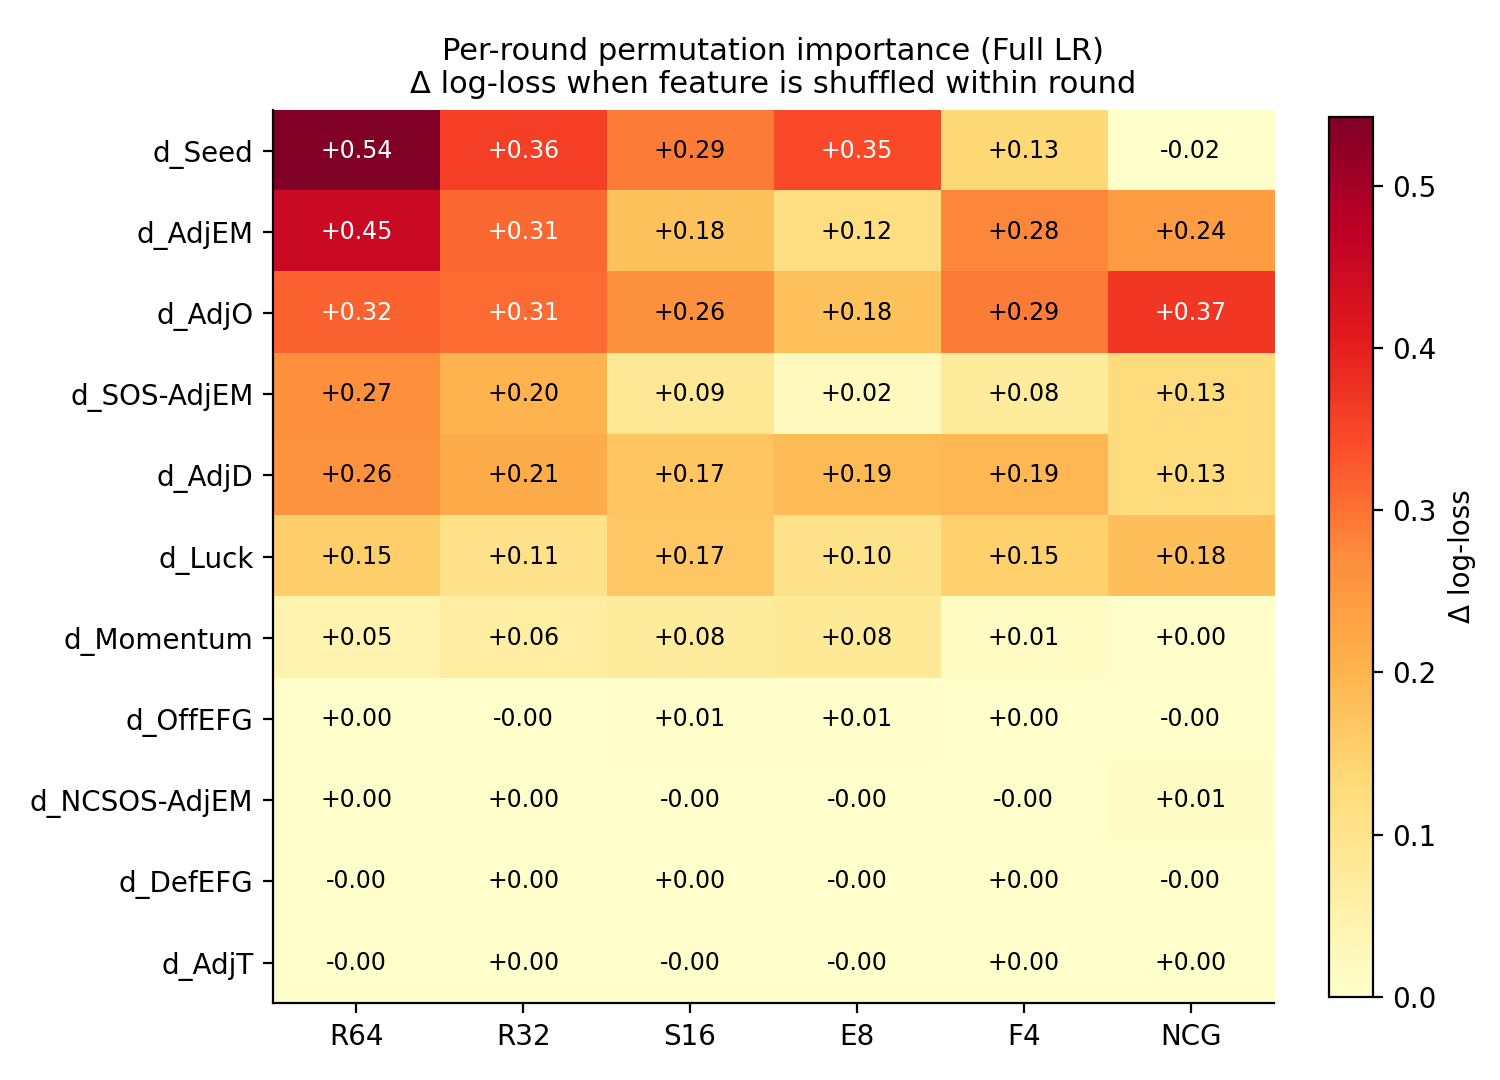
\includegraphics[width=0.7\textwidth]{figures/round_importance.png}
\caption{Round-by-round standardized coefficient magnitudes for separately fit logistic regressions.}
\label{fig:rounds}
\end{figure}

\subsection{Vectorized Monte Carlo simulator}

Instead of running the 63 games per replicate through the model, we build the $64\times 64$ matrix $P_{ij} = P_\theta(i\text{ beats }j)$ once per season, and during each replicate sample 63 Bernoulli draws against the precomputed lookup tables. This brings the per-replicate complexity to $O(n_{\text{sims}} \cdot 63)$, with a one-time precomputation cost of $O(64^2)$. With $n_{\text{sims}} = 10{,}000$, the simulated results are computed in seconds, with the per-team qualifying probabilities having a standard error of less than one percentage point.

\section{Results}

\subsection{Historical backtest (2010--2026, $n=15$)}

For each season, we train the model on all other seasons (strict LOSO, no leakage), yielding the chalk\_seed and chalk\_model brackets that we would compare against the actual outcome. The full season-by-season comparison is shown in Figure~\ref{fig:backtest}. Summary statistics:

\begin{itemize}[leftmargin=*]
\item The model bracket beats the seed in \textbf{13 out of 15 tournaments} (binomial $p \approx 0.004$).
\item Mean score: chalk\_seed \textbf{827}, chalk\_model \textbf{1{,}255}, $\Delta = +428$ ($52\%$ relative improvement).
\item The two losses are 2017 (a chalky North Carolina--Gonzaga championship) and 2025 (an exceptionally chalky tournament where seed-chalk scored 1{,}730).
\item The model never \emph{expects} chalk\_seed to outperform: $\mathbb{E}[\text{model}] > \mathbb{E}[\text{seed}]$ in 15 of 15 seasons.
\end{itemize}

A useful internal check: the model's mean expected score over seasons (1{,}250.5) closely matches the model's realized mean score (1{,}255.3), indicating no systematic bias in the estimated probabilities.

\begin{figure}[H]
\centering
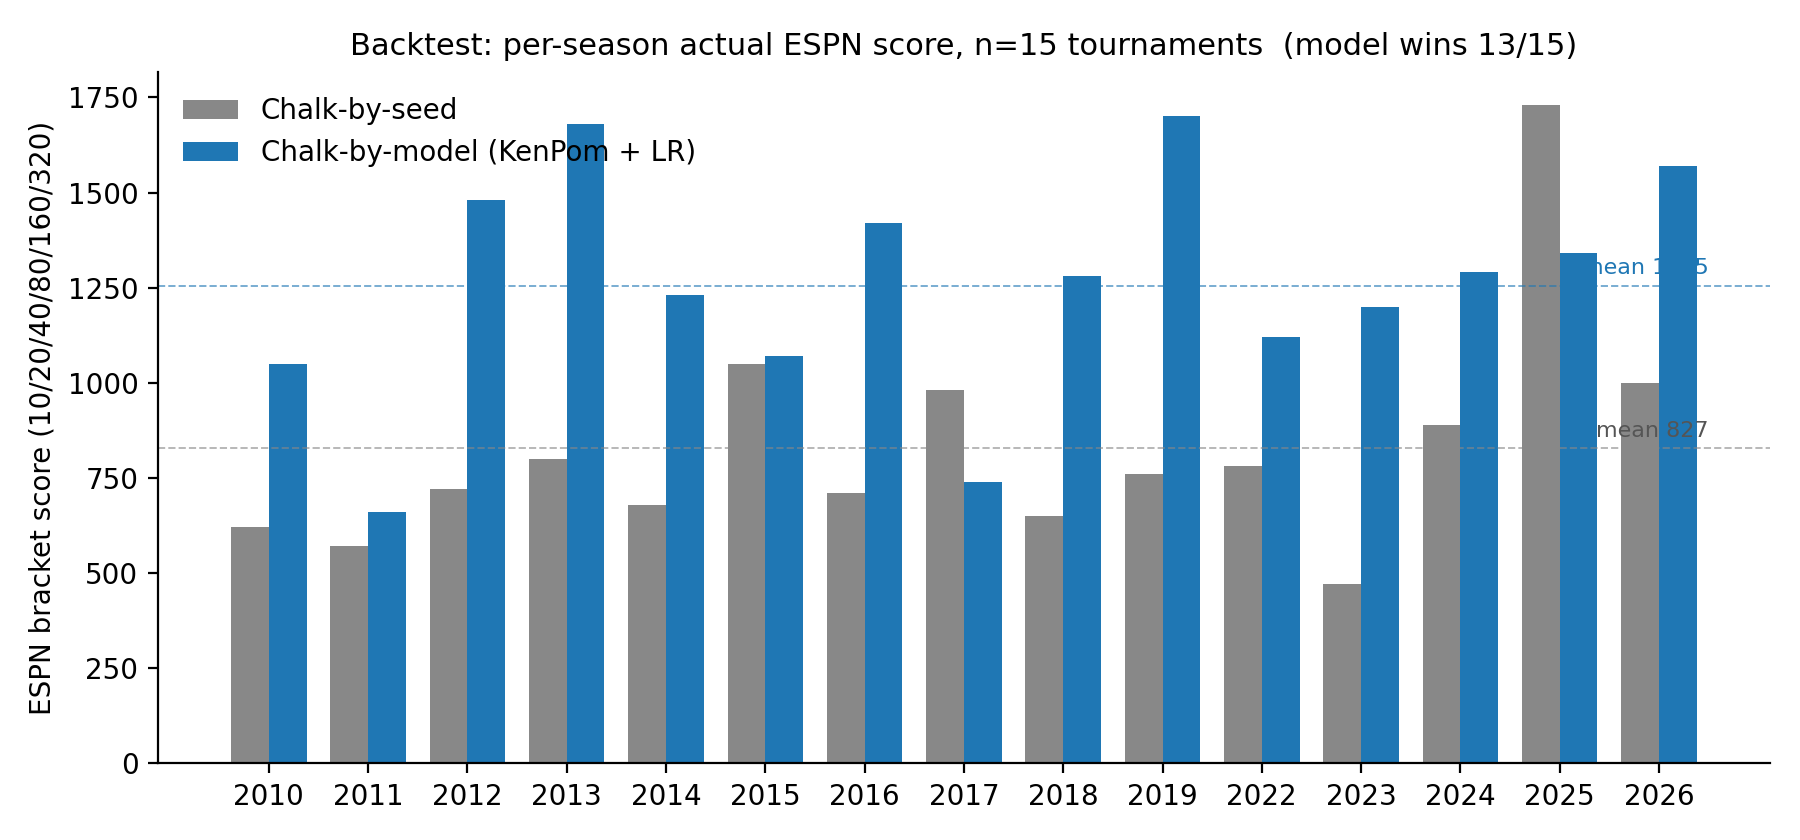
\includegraphics[width=0.8\textwidth]{figures/backtest.png}
\caption{Per-season actual ESPN score, chalk-by-seed vs.\ chalk-by-model, 2010--2026 (excluding 2020).}
\label{fig:backtest}
\end{figure}

\subsection{The 2026 tournament --- predictions}

The model projected a heavy favorite in Michigan. Champion probabilities for the top teams (see full reach-probability heatmap in Figure~\ref{fig:reach}):

\begin{table}[H]
\centering
\begin{tabular}{lcrr}
\toprule
Team & Seed & $P(\text{Champion})$ & $P(\text{F4})$ \\
\midrule
Michigan & 1 & \textbf{0.672} & 0.970 \\
Arizona & 1 & 0.253 & 0.914 \\
Duke & 1 & 0.069 & 0.839 \\
Illinois & 3 & 0.003 & 0.434 \\
Connecticut & 2 & 0.000 & 0.101 \\
\bottomrule
\end{tabular}
\caption{Top 2026 reach probabilities under the trained model.}
\end{table}

A $67.2\%$ champion probability is unusually concentrated for any single team. The model miss on the eventual runner-up Connecticut, who had near-zero champion probability, is partially compensated for by the Monte Carlo simulation, which considers all possible tournament paths.

\begin{figure}[H]
\centering
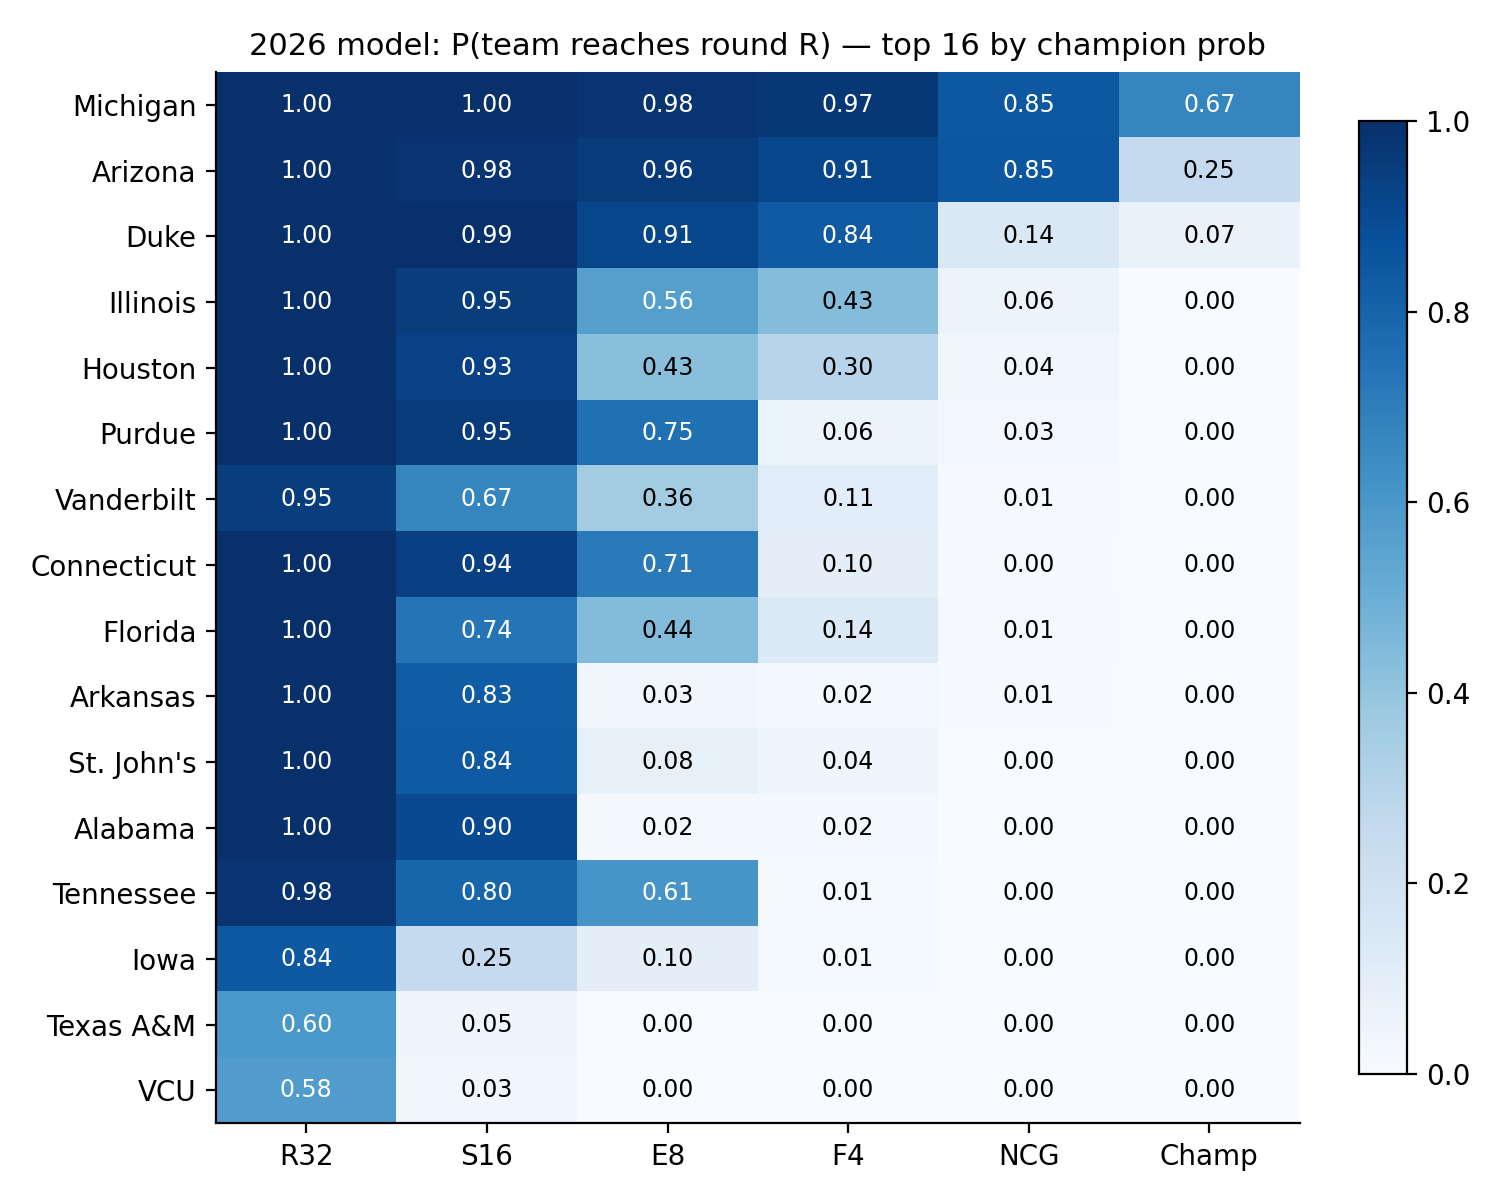
\includegraphics[width=0.7\textwidth]{figures/reach_2026.png}
\caption{2026 reach probability heatmap for the top 16 teams by champion probability.}
\label{fig:reach}
\end{figure}

\subsection{The 2026 tournament --- outcome and strategy scores}

Michigan won the championship, defeating Connecticut 69-63. Upsets of the tournament included Iowa (9) over Florida (1), Texas (11) over Gonzaga (3), and Connecticut (2) defeating Duke (1) in the E8.

\begin{table}[H]
\centering
\begin{tabular}{lrrrrrrr}
\toprule
Strategy & Total & R64 & R32 & S16 & E8 & F4 & NCG \\
\midrule
chalk\_seed & 1{,}000 & 240 & 240 & 200 & 160 & 160 & 0 \\
chalk\_model & \textbf{1{,}570} & 310 & 260 & 280 & 240 & 160 & 320 \\
ev\_max & \textbf{1{,}570} & 310 & 260 & 280 & 240 & 160 & 320 \\
\bottomrule
\end{tabular}
\caption{2026 strategy scores broken out by round.}
\end{table}

The models both decisively outperform chalk\_seed (+570 each), correctly picking Michigan as the champion. chalk\_model and ev\_max make the same predictions for all 63 games, confirming the closed-form equivalence shown in \S3.3.

\subsection{Distributional analysis}

In 10{,}000 simulated tournaments using the 2026 model:

\begin{table}[H]
\centering
\begin{tabular}{lrrrrr}
\toprule
Strategy & Mean & SD & p10 & Median & p90 \\
\midrule
chalk\_seed & 1{,}301 & 191 & 1{,}060 & 1{,}290 & 1{,}590 \\
\textbf{chalk\_model} & \textbf{1{,}528} & \textbf{222} & \textbf{1{,}210} & \textbf{1{,}600} & \textbf{1{,}780} \\
ev\_max & 1{,}528 & 222 & 1{,}210 & 1{,}600 & 1{,}780 \\
\bottomrule
\end{tabular}
\caption{Score distributions for each strategy across 10{,}000 simulated 2026 tournaments.}
\end{table}

The model strategies also have a \textbf{{+227}-point expected score advantage} and slightly larger variance (Figure~\ref{fig:strategy}). The larger variance is by design: concentrating our picks on a high-probability champion increases both the mean and the right-tail of the score distribution.

\begin{figure}[H]
\centering
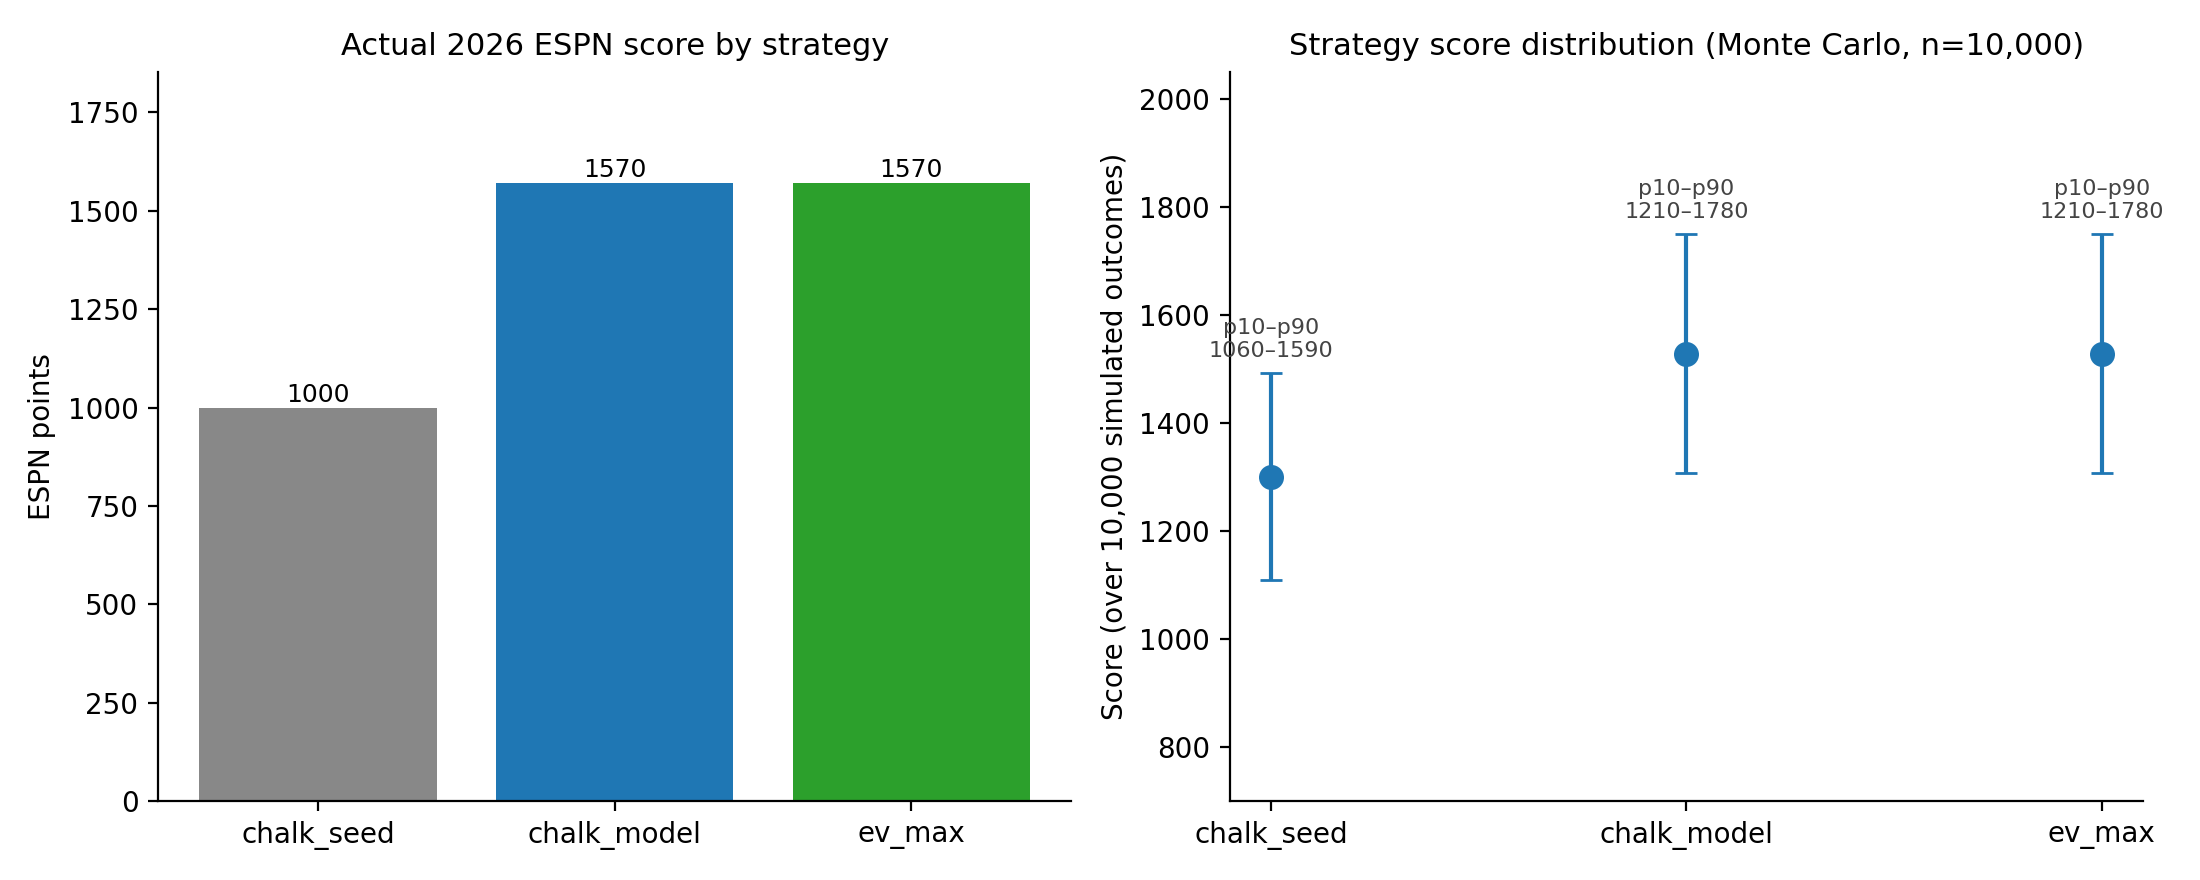
\includegraphics[width=0.8\textwidth]{figures/strategy_2026.png}
\caption{2026 strategy comparison. Left: realized ESPN score. Right: distribution over 10{,}000 simulated outcomes.}
\label{fig:strategy}
\end{figure}

\section{Discussion}

Three general points arise. First, calibration is more important than marginal accuracy. The full LR is still slightly better than tree ensembles with respect to log-loss and Brier score, both relevant for expected value decisions. When decisions depend on probability \emph{magnitudes}, a well-calibrated linear model can outperform a higher-accuracy non-linear one---this is the gap between predicting winners and estimating probabilities you can actually compute expectations against.

Nonlinear scoring increases model confidence. In 2026, the model's strong belief in Michigan produces a champion distribution sharply concentrated on Michigan and a well-performing bracket. The backtest confirms this: the difference between the model and seed reflects tournament "chalkiness".

\textbf{The EV optimization collapses to a greedy rule.} What looks like a $2^{63}$-element search problem is solved by inspection given a fixed model: at every node, pick the team with higher reach probability. The hard work has been pushed into the calibration of the model---exactly where modeling effort should sit. The downside of this greediness is that EV maximization and pool-percentile maximization are not the same. The leverage strategy from \S3.5 provides a tractable theoretical bridge, and future multi-year public-pick data could sharpen it.

\section{Improvements}

The key limitations relate to what data is available: only single-year (2019) public-pick data is available for pool-percentile optimization. Additionally, late-season injuries, suspensions, and styles of play for potential matchups could not be included in these ratings. The small (63 games/year $\times$ 15 year) dataset prevents observing complicated patterns (but these are properties of the tournament data, not limitations of the approach).

Extensions include game-log scraping for all KenPom-rated teams (enabling conference-tournament margin of victory and obviating the Momentum proxy), multi-year public-pick scraping to back-test the \S3.5 leverage heuristic, PFP optimization via simulated annealing directly on the bracket space, directly learning $\boldsymbol{\theta}$ to maximize expected bracket EV instead of minimizing the log-loss, via policy-gradient or differentiable simulation, and round-specific feature weights, motivated by the round-by-round fits reported in \S4.2, which suggest feature importance varies as the tournament progresses.

\section{Conclusions}

We built an end-to-end NCAA tournament prediction pipeline comprised of data collection, a calibrated model of win probability, a vectorized Monte Carlo simulation, and three deterministic bracket-building strategies. In backtesting, the model bracket scores $52\%$ more ESPN points than the seed-chalk bracket on average and wins 13 out of 15 past tournaments. For 2026, the model bracket scored 1{,}570 to 1{,}000 for seed-chalk, predicting Michigan would win with a success probability of $67.2\%$.

Two methodological observations: since the EV objective decomposes by linearity of expectation, the entry that is EV-maximizing under the fixed model gives a \emph{closed-form greedy} solution. Most ``optimization'' formulations of bracket selection ignore that exponential search is not necessary. A simple example is that chalk\_model and ev\_max agree on every decision for all 63 2026 games. Second, the gap between EV maximization and pool-percentile maximization is real and persistent, and the leverage heuristic of \S3.5 is a tractable theoretical bridge for future work.

In a class on discrete modeling and Monte Carlo simulation, this project viewed the bracket as a depth-six binary tree, the win-probability model as the per-edge transition kernel, and Monte Carlo methods as the only way to calculate the resulting joint distribution.

\section*{Acknowledgments}

We thank Prof.\ Tim Chartier for the project framing and for sharing access to KenPom.com, which provided the team efficiency ratings used throughout this work. We also thank Sports Reference LLC for the tournament results and per-game schedule data.

\begin{thebibliography}{99}

\bibitem{kenpom}
K.\ Pomeroy, \emph{KenPom College Basketball Ratings}, kenpom.com, accessed 2026.

\bibitem{sportsref}
Sports Reference LLC, \emph{NCAA Men's Tournament Brackets and Schedules}, sports-reference.com/cbb, accessed 2026.

\bibitem{sklearn}
F.\ Pedregosa et al., ``Scikit-learn: Machine Learning in Python,'' \emph{Journal of Machine Learning Research}, vol.\ 12, pp.\ 2825--2830, 2011.

\bibitem{xgboost}
T.\ Chen and C.\ Guestrin, ``XGBoost: A Scalable Tree Boosting System,'' in \emph{Proc.\ KDD '16}, 2016, pp.\ 785--794.

\bibitem{lightgbm}
G.\ Ke et al., ``LightGBM: A Highly Efficient Gradient Boosting Decision Tree,'' in \emph{NeurIPS 2017}, pp.\ 3149--3157.

\bibitem{catboost}
L.\ Prokhorenkova et al., ``CatBoost: unbiased boosting with categorical features,'' in \emph{NeurIPS 2018}.

\bibitem{lopezmatthews}
M.\ J.\ Lopez and G.\ J.\ Matthews, ``Building an NCAA men's basketball predictive model and quantifying its success,'' \emph{Journal of Quantitative Analysis in Sports}, vol.\ 11, no.\ 1, 2015.

\bibitem{metrick}
A.\ Metrick, ``March Madness? Strategic behavior in NCAA basketball tournament betting pools,'' \emph{Journal of Economic Behavior \& Organization}, vol.\ 30, no.\ 2, pp.\ 159--172, 1996.

\bibitem{espn}
``26.6 Million Brackets! ESPN Tournament Challenge Sets New Record for Fourth Consecutive Year,'' \emph{ESPN Press Room}, March 26, 2026. \url{https://espnpressroom.com/us/press-releases/2026/03/26-6-million-brackets-espn-tournament-challenge-sets-new-record-for-fourth-consecutive-year/}

\end{thebibliography}

\end{document}